
Le kendo est un art traditionnel chinois qui se pratique avec un shinai, sabre en bambou. Ci-dessous, on a représneté par un diagramme en boite portant sur la masse (en g) un échantillon de shinais fabriqué par le fabricant Kumamoto.

\begin{center}
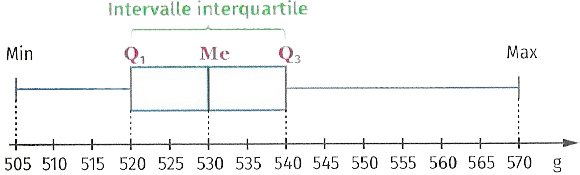
\includegraphics[scale=1]{stat-30.jpg}
\end{center}


\begin{enumerate}
\item Lire la valeur de la médiane.
\item Écrire trois phrases commençant par : "Environ 50\% des shinais ont une masse comprise entre ..."
\item Calculer l'écart interquartile.
\item Pour être homologué, la masse d'un shinai doit être supérieur à 510 g. Que penser de la production de Kumamoto ?
\end{enumerate} 